% Chapter 19. The combination that turns an inconvenience into a breach.
\documentclass[tikz,border=6pt]{standalone}
% Shared look for every TikZ figure in the book.
% Colours match book/preamble.tex exactly. Change both or neither.

\usepackage{tikz}
\usepackage{xcolor}
\usepackage{amsmath}
\IfFileExists{libertinus.sty}{\usepackage[mono=false]{libertinus}}{}
\IfFileExists{inconsolata.sty}{\usepackage[varqu,varl,scaled=0.95]{inconsolata}}{}

\usetikzlibrary{
  arrows.meta, positioning, calc, fit, backgrounds, shapes.geometric,
  shapes.misc, decorations.pathreplacing, decorations.pathmorphing,
  patterns, chains, matrix, shadows.blur
}

\definecolor{ink}{HTML}{15181D}
\definecolor{muted}{HTML}{5B6472}
\definecolor{rule}{HTML}{C9CED6}
\definecolor{wash}{HTML}{F4F5F7}
\definecolor{accent}{HTML}{0F5C8C}
\definecolor{accentsoft}{HTML}{E7F0F6}
\definecolor{warm}{HTML}{B4531A}
\definecolor{warmsoft}{HTML}{FBF0E7}
\definecolor{good}{HTML}{2C6E49}
\definecolor{goodsoft}{HTML}{E9F2EC}
\definecolor{danger}{HTML}{9B2226}
\definecolor{dangersoft}{HTML}{FAECEC}

\tikzset{
  font=\sffamily\small,
  >={Stealth[length=5pt, width=4pt]},
  %
  box/.style={
    draw=rule, line width=0.8pt, fill=wash, rounded corners=2pt,
    inner sep=7pt, align=center, text=ink, minimum height=9mm,
  },
  boxa/.style={box, draw=accent, fill=accentsoft},
  boxg/.style={box, draw=good,   fill=goodsoft},
  boxw/.style={box, draw=warm,   fill=warmsoft},
  boxd/.style={box, draw=danger, fill=dangersoft},
  %
  lane/.style={draw=rule, line width=0.7pt, fill=white, rounded corners=2pt,
               inner sep=6pt, align=center, minimum width=26mm},
  %
  flow/.style={draw=accent, line width=1.0pt, ->},
  flowback/.style={flow, densely dashed},
  flowmuted/.style={draw=muted, line width=0.8pt, ->},
  lifeline/.style={draw=rule, line width=0.7pt, densely dotted},
  %
  lbl/.style={font=\sffamily\scriptsize, text=muted, inner sep=2pt},
  lblink/.style={font=\sffamily\scriptsize, text=ink, inner sep=2pt},
  tag/.style={font=\ttfamily\scriptsize, text=accent, inner sep=2pt,
              fill=white, inner xsep=3pt},
  note/.style={font=\sffamily\scriptsize\itshape, text=muted, align=left},
  %
  band/.style={draw=none, rounded corners=1pt},
  tick/.style={draw=muted, line width=0.6pt},
}

% A horizontal timeline bar segment: \barseg{x0}{x1}{y}{colour}{label}
\newcommand{\barseg}[5]{%
  \fill[#4, rounded corners=1pt] (#1,#3-0.16) rectangle (#2,#3+0.16);
  \node[lbl, text=white, font=\sffamily\scriptsize\bfseries]
       at ({(#1+#2)/2},#3) {#5};
}

\begin{document}
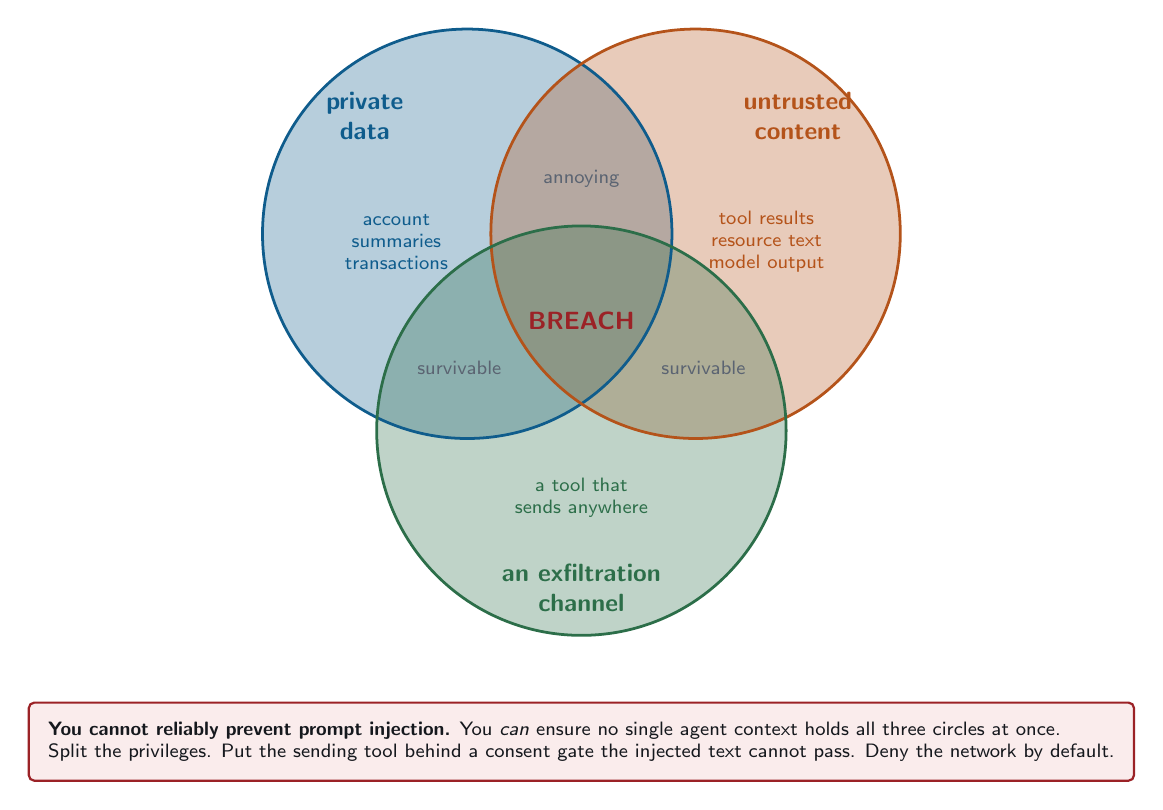
\begin{tikzpicture}[x=1cm, y=1cm]

  \def\R{2.6}

  \begin{scope}[opacity=0.30]
    \fill[accent] (-1.45,0.85) circle (\R);
    \fill[warm]   ( 1.45,0.85) circle (\R);
    \fill[good]   ( 0.00,-1.65) circle (\R);
  \end{scope}

  \draw[draw=accent, line width=1pt] (-1.45,0.85) circle (\R);
  \draw[draw=warm,   line width=1pt] ( 1.45,0.85) circle (\R);
  \draw[draw=good,   line width=1pt] ( 0.00,-1.65) circle (\R);

  \node[align=center, font=\sffamily\small\bfseries, text=accent]
    at (-2.75,2.35) {private\\data};
  \node[align=center, font=\sffamily\small\bfseries, text=warm]
    at (2.75,2.35) {untrusted\\content};
  \node[align=center, font=\sffamily\small\bfseries, text=good]
    at (0,-3.65) {an exfiltration\\channel};

  \node[align=center, font=\sffamily\scriptsize, text=accent]
    at (-2.35,0.75) {account\\summaries\\transactions};
  \node[align=center, font=\sffamily\scriptsize, text=warm]
    at (2.35,0.75) {tool results\\resource text\\model output};
  \node[align=center, font=\sffamily\scriptsize, text=good]
    at (0,-2.5) {a tool that\\sends anywhere};

  % pairwise intersections
  \node[align=center, font=\sffamily\scriptsize, text=muted] at (0,1.55)
    {annoying};
  \node[align=center, font=\sffamily\scriptsize, text=muted] at (-1.55,-0.85)
    {survivable};
  \node[align=center, font=\sffamily\scriptsize, text=muted] at (1.55,-0.85)
    {survivable};

  % the centre
  \node[align=center, font=\sffamily\small\bfseries, text=danger] at (0,-0.25)
    {BREACH};

  \node[boxd, minimum width=132mm, align=left, font=\sffamily\scriptsize]
    at (0,-5.6)
    {\textbf{You cannot reliably prevent prompt injection.} You \emph{can}
     ensure no single agent context holds all three circles at once.\\
     Split the privileges. Put the sending tool behind a consent gate the
     injected text cannot pass. Deny the network by default.};

\end{tikzpicture}
\end{document}
